\documentclass[12pt]{article}

\usepackage{sbc-template}
\usepackage{graphicx,url}
\usepackage[utf8]{inputenc}
% Para hifenização correta em português na versão final, instale o suporte
% (ex.: apt-get install texlive-lang-portuguese) e reative a linha abaixo:
\usepackage[brazil]{babel}
\usepackage{booktabs}
\usepackage{amsmath}

\sloppy

\title{Previsão do Retorno do Café Arábica (KC=F) com Redes LSTM\\
e Variáveis Climáticas Regionais de Minas Gerais}

\author{Euler G. Rocha\inst{1}, Antonio A. Ambrosio\inst{1}, Marcos R. Ribeiro\inst{1}}

\address{Instituto Federal de Minas Gerais (IFMG) -- Campus Bambuí\\
  Bambuí -- MG -- Brasil
  \email{eulergomesrocha@gmail.com}
}

\begin{document}

\maketitle

\begin{abstract}
  We forecast the one-day-ahead log-return of arabica coffee futures (KC=F) with
  LSTM networks that combine market indicators and daily climate observations from
  four INMET stations in the main producing regions of Minas Gerais, Brazil.
  Using a leakage-controlled walk-forward protocol (expanding window, embargo,
  per-fold scaling) and a five-seed ensemble, we benchmark against a random walk,
  ARIMA and GARCH, and test significance with the Diebold--Mariano test. No model
  significantly beats the random walk --- an honest result for a daily commodity
  return. Adding climate reduces RMSE marginally, and a per-city representation
  outperforms a production-weighted aggregate, suggesting that regional
  granularity carries useful signal, albeit within seed noise.
\end{abstract}

\begin{resumo}
  Prevemos o log-retorno de um dia à frente dos futuros de café arábica (KC=F) com
  redes LSTM que combinam indicadores de mercado e observações climáticas diárias de
  quatro estações do INMET nas principais regiões produtoras de Minas Gerais.
  Empregando um protocolo walk-forward com controle de vazamento (janela expansiva,
  embargo, normalização por fold) e um ensemble de cinco sementes, comparamos com
  random walk, ARIMA e GARCH, e testamos significância com Diebold--Mariano. Nenhum
  modelo supera o random walk de forma significativa --- resultado honesto para
  retornos diários de commodity. Adicionar clima reduz marginalmente o RMSE, e a
  representação por cidade supera a agregação ponderada por produção, sugerindo que a
  granularidade regional carrega sinal útil, ainda que dentro do ruído de semente.
\end{resumo}

\section{Introdução}


O Brasil é o maior produtor e exportador mundial de café, e Minas Gerais responde
pela maior parte da produção nacional de café arábica \cite{CONAB2025}. A volatilidade do preço da
commodity afeta diretamente produtores, cooperativas, exportadores e investidores, de modo que
previsões confiáveis podem apoiar decisões ao longo de toda a cadeia produtiva. Além de fatores econômicos,
eventos climáticos extremos, como geadas, secas e ondas de calor, influenciam significativamente a produtividade das lavouras e, 
consequentemente, a formação dos preços no mercado futuro.

Diferentemente da maioria das abordagens de previsão financeira, que se apoiam apenas em indicadores de mercado,
este trabalho investiga a utilização de variáveis climáticas regionais como fonte complementar de informação. 
Embora modelos baseados em aprendizado profundo, como redes \emph{Long Short-Term Memory} (LSTM), tenham sido amplamente aplicados
à previsão de séries temporais financeiras, ainda há poucas investigações sobre o impacto da granularidade espacial das informações
climáticas na previsão dos retornos diários do café arábica.

Este trabalho investiga se a incorporação de variáveis climáticas regionais melhora a 
previsão do retorno diário dos contratos futuros de café arábica (KC=F), negociados na ICE,
por meio de redes \emph{Long Short-Term Memory} (LSTM). As contribuições são: (i) a construção de um conjunto
de dados que alinha o preço do KC=F, o câmbio BRL/USD e observações diárias de quatro estações automáticas 
do INMET nas principais regiões cafeeiras de Minas Gerais; (ii) um protocolo de avaliação temporal rigoroso,
com controle explícito de vazamento de dados, validação walk-forward e teste de significância; e (iii) uma análise da
contribuição das variáveis climáticas, incluindo uma comparação entre sua representação \emph{por cidade} (granularidade regional) e 
uma representação \emph{agregado ponderado pela produção}.

Antecipamos o principal achado: em log-retorno diário, nenhum modelo (LSTM, ARIMA ou 
GARCH) supera o Random Walk de forma estatisticamente significativa, resultado compatível 
com a elevada eficiência do mercado nesse horizonte temporal. Ainda assim, a inclusão das variáveis
climáticas reduz marginalmente o erro de previsão e a representação por cidade apresenta desempenho
superior à agregação ponderada, indicando que a preservação da granularidade regional mantém informações 
úteis para a modelagem preditiva.


\section{Materiais}

\subsection{Fontes de dados}

O preço de fechamento diário do KC=F (em USD/lb) e a taxa de câmbio BRL/USD foram
obtidos via \texttt{yfinance} (Yahoo Finance). As variáveis climáticas vêm da rede de
estações automáticas do INMET (BDMEP)~\cite{inmet2025bdmep}, consolidadas de frequência
horária para diária.
Foram usadas quatro estações, representando três regiões produtoras
(Tabela~\ref{tab:estacoes}).

\begin{table}[ht]
\centering
\caption{Estações INMET utilizadas e respectivas microrregiões.}
\label{tab:estacoes}
\begin{tabular}{llrl}
\toprule
Cidade & Código & Altitude & Região \\
\midrule
Varginha   & A515 & 942 m & Sul de Minas \\
Machado    & A567 & 871 m & Sul de Minas \\
Patrocínio & A523 & 931 m & Cerrado Mineiro \\
Manhuaçu   & A556 & 674 m & Matas de Minas \\
\bottomrule
\end{tabular}
\end{table}

De cada estação retêm-se temperatura média, máxima e mínima do ar, precipitação total,
radiação solar global, umidade relativa média, velocidade e rajada do vento, além de
um indicador de risco de geada (temperatura mínima $<0\,^{\circ}$C) e uma medida de
\emph{graus-frio} acumulados. O conjunto final cobre 1.763 pregões entre 31/12/2018 e
30/12/2025.

\subsection{Análise exploratória}

O nível do preço é fortemente não estacionário (ADF $p=0{,}80$), enquanto o
log-retorno $r_t = \ln(P_t/P_{t-1})$ é estacionário (ADF $p\approx 0$), o que motiva
modelar o retorno. Os log-retornos são quase simétricos (assimetria $0{,}08$) e
levemente leptocúrticos (curtose em excesso $0{,}74$), com volatilidade anualizada de
$35{,}9\%$. A autocorrelação da \emph{média} dos retornos é fraca (ACF/PACF dentro das
bandas, Figura~\ref{fig:acf}), mas a dos retornos ao quadrado é significativa e
persistente, evidência de \emph{volatility clustering}.

\begin{figure}[ht]
\centering
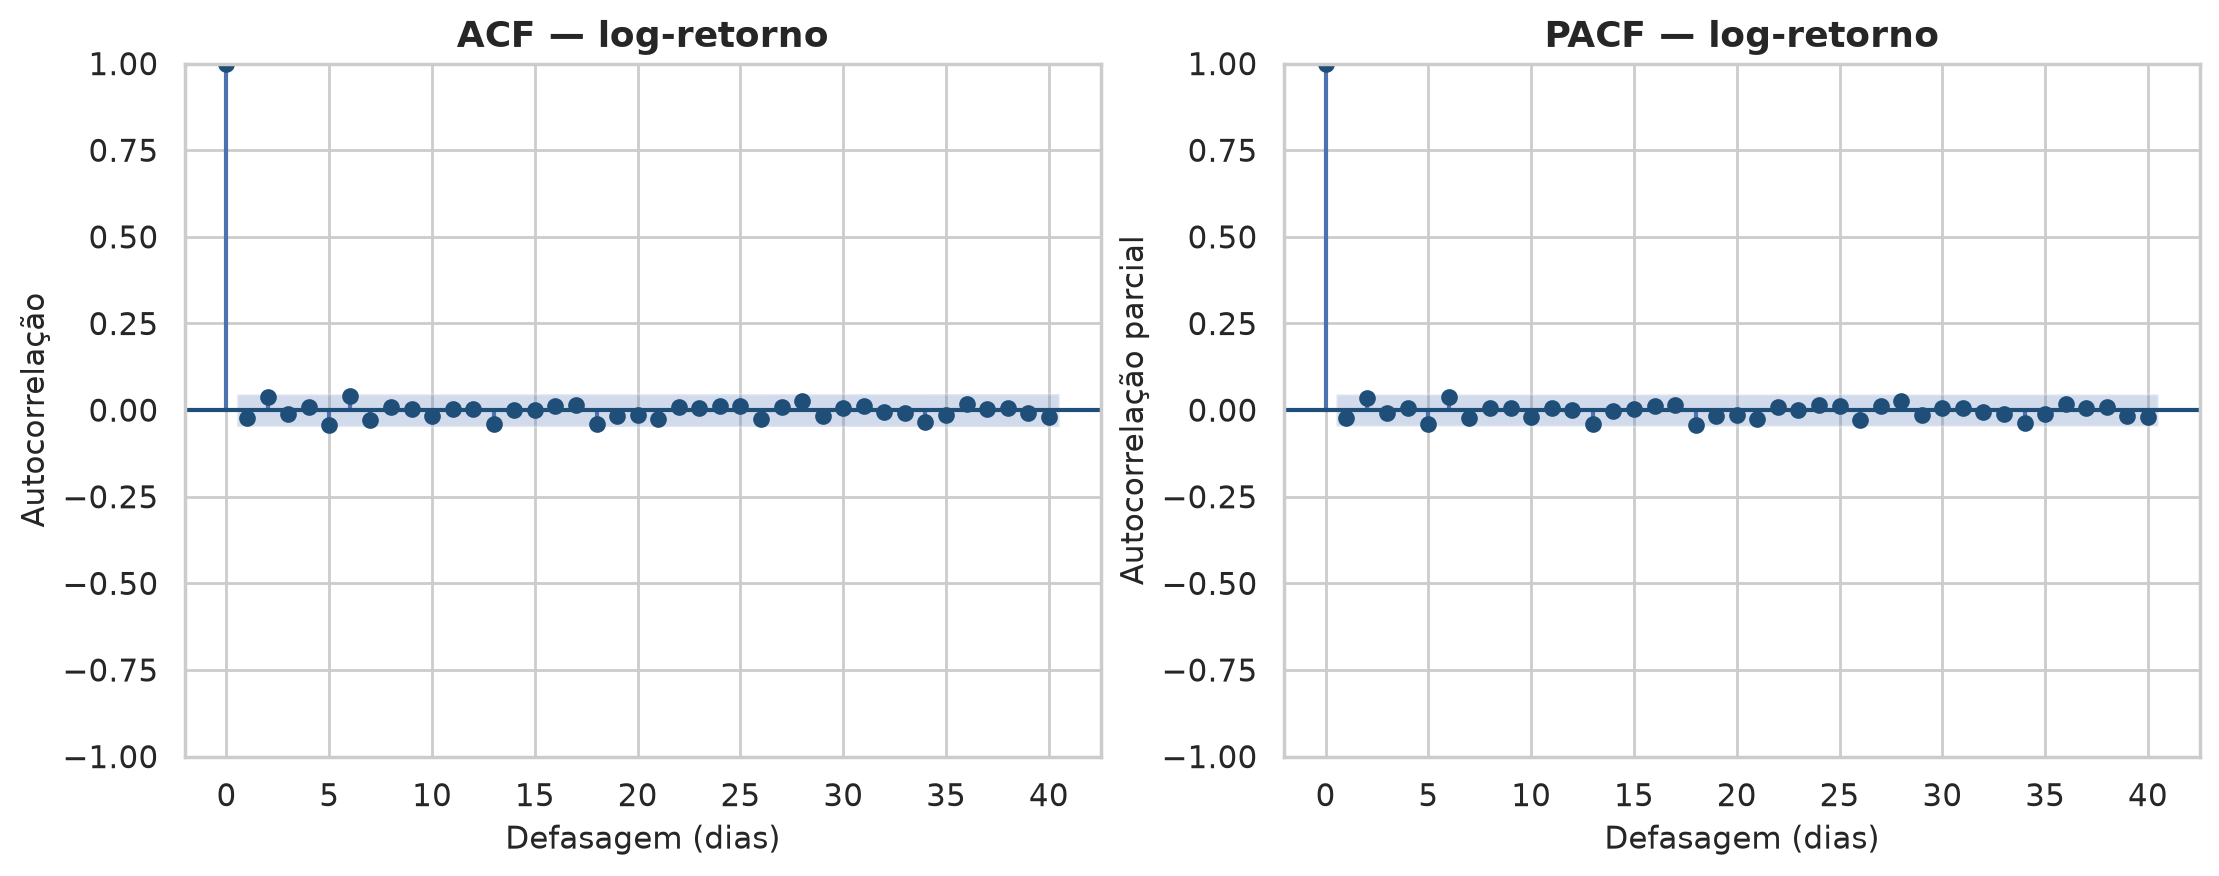
\includegraphics[width=.9\textwidth]{fig_acf.png}
\caption{ACF e PACF do log-retorno: pouca autocorrelação linear na média, sugerindo
ordens baixas de ARIMA e ganho preditivo, se houver, em estrutura não linear/exógena.}
\label{fig:acf}
\end{figure}

Eventos de risco de geada são raros e concentrados no inverno, sobretudo em Patrocínio
(19 dias) e Varginha (12), contra Machado (3) e Manhuaçu (1) --- 23 dias com pelo menos
uma estação em risco na amostra. A correlação linear contemporânea entre clima e
log-retorno é praticamente nula; contudo, o retorno médio nas semanas seguintes a um dia
de risco de geada supera o de dias normais, sugerindo um efeito \emph{defasado} e não
instantâneo (Figura~\ref{fig:geada}). Isso justifica o uso de janelas temporais e de
variáveis climáticas acumuladas.

\begin{figure}[ht]
\centering
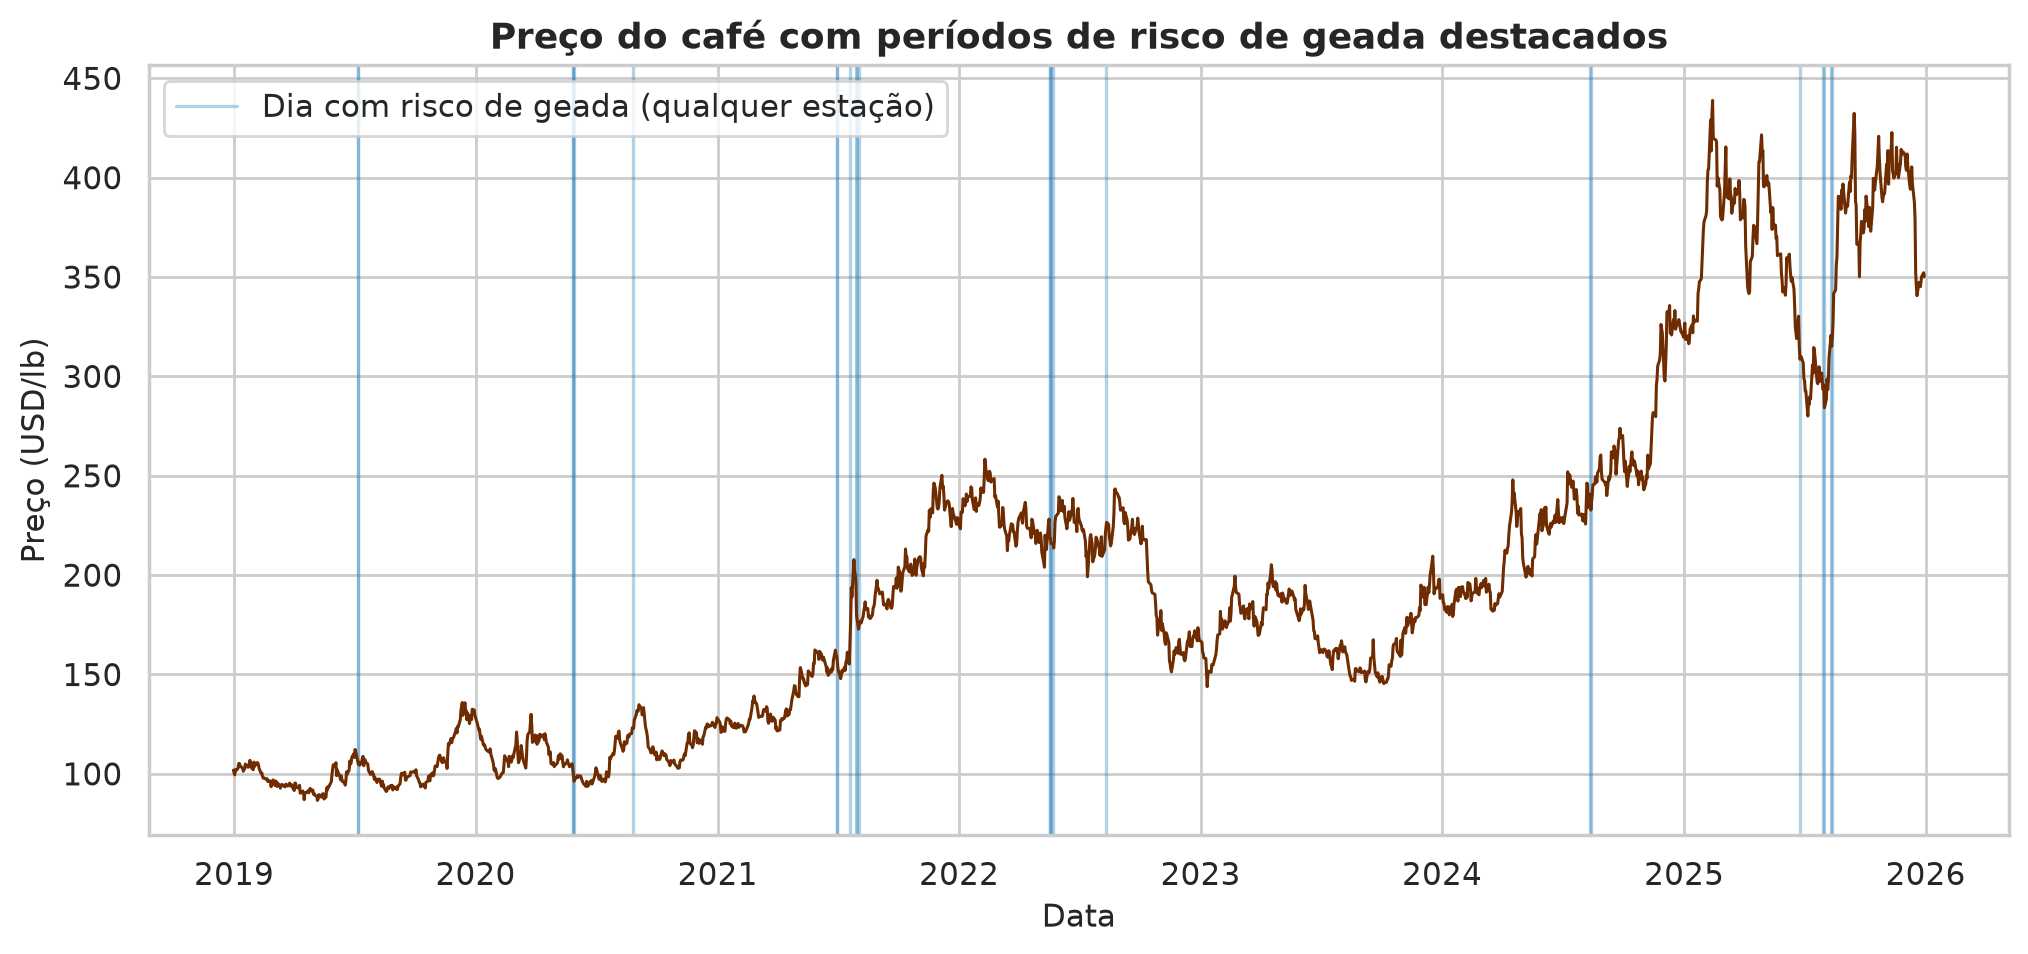
\includegraphics[width=.9\textwidth]{fig_preco_geada.png}
\caption{Preço do café com dias de risco de geada destacados. Episódios (notadamente em
2021) coincidem com movimentos de alta, sugerindo reprecificação defasada da oferta futura.}
\label{fig:geada}
\end{figure}

\section{Metodologia}

\subsection{Alvo e atributos}

O alvo é o log-retorno de um dia à frente. Além do próprio retorno e do retorno do
câmbio, computam-se atributos de mercado (volatilidades de 5 e 21 dias, média móvel de
10 dias) e de sazonalidade ($\sin$ e $\cos$ do dia do ano). Avaliam-se quatro
configurações de atributos: \textbf{(a)} apenas mercado (sem clima); e três formas de
incorporar o clima --- \textbf{(b) Opção B}, clima bruto \emph{por cidade} (formato
\emph{wide}, cada estação com suas colunas); \textbf{(c)} clima defasado/acumulado
(risco de geada agregado e graus-frio em janelas de 30 dias); e \textbf{(d) Opção C}, em
que cada variável climática é substituída por uma única \emph{média ponderada pela
produção} das regiões. Os pesos derivam da participação da produção de arábica de Minas
Gerais (Sul de Minas $\approx 55\%$, Matas de Minas $\approx 25\%$, Cerrado Mineiro
$\approx 15\%$; fontes IBGE e EMATER-MG), resultando em Varginha $0{,}29$, Machado
$0{,}29$, Manhuaçu $0{,}26$ e Patrocínio $0{,}16$.

\subsection{Protocolo de validação temporal}

Cada amostra é uma janela de \textsc{lookback}${}=45$ dias de atributos que prevê o
retorno do dia seguinte. Usa-se validação \emph{walk-forward} com janela de treino
\emph{expansiva} (5 folds a partir de 50\% dos dados). Entre treino e teste aplica-se um
\emph{embargo} de 45 dias, garantindo que nenhuma janela de teste contenha dias já
vistos no treino. Em cada fold, o \texttt{StandardScaler} e a seleção de atributos são
ajustados \emph{apenas} no núcleo de treino (85\% inicial; os 15\% finais servem de
validação para \emph{early stopping}), eliminando vazamento.

\subsection{Modelo e robustez}

A rede é uma LSTM~\cite{hochreiter1997lstm} de uma camada (48 unidades, \emph{dropout}
$0{,}2$) seguida de uma camada linear, otimizada com Adam~\cite{kingma2015adam}
($\text{lr}=10^{-3}$, \emph{weight decay} $10^{-4}$) e \emph{early stopping}. Para controlar o efeito da inicialização aleatória, cada
configuração é treinada com \textbf{5 sementes por fold} e avaliada como \emph{ensemble}
(média das previsões); reporta-se também a dispersão do RMSE entre sementes.

\subsection{Baselines e métricas}

Comparamos com três baselines sob o mesmo protocolo e nos mesmos dias-alvo:
\textbf{random walk} ($\hat{r}_t = 0$), \textbf{ARIMA}~\cite{box1976time} (ordem
escolhida por AIC no treino, previsão recursiva de um passo sem \emph{refit}) e
\textbf{GARCH(1,1)}~\cite{bollerslev1986generalized} como baseline de
\emph{volatilidade}. As métricas de nível são RMSE, MAE, sMAPE, MASE~\cite{hyndman2006another}
e acurácia direcional; a significância estatística é avaliada pelo teste de
Diebold--Mariano (DM)~\cite{diebold1995comparing}, com a convenção $\mathrm{DM}<-1{,}96$
indicando modelo significativamente melhor que a referência. A seleção de atributos usa
a importância de um \emph{Random Forest}~\cite{breiman2001random} treinado dentro do
fold, reportando-se a estabilidade (frequência no top-12 entre os folds).

\section{Resultados e Discussão}

A Tabela~\ref{tab:comparativa} resume o desempenho. Random walk e ARIMA empatam em RMSE
($0{,}02325$), confirmando a expectativa da análise exploratória de que a média dos
retornos é quase imprevisível. A LSTM apenas com mercado é \emph{significativamente
pior} que o random walk ($\mathrm{DM}_{oos}=2{,}51$). A inclusão de clima bruto por
cidade (Opção B) reduz o RMSE para $0{,}02345$, recupera o empate com o random walk
($\mathrm{DM}_{oos}=1{,}12$, não significativo) e é a única configuração de LSTM com
acurácia direcional acima do acaso ($0{,}502$).

\begin{table}[ht]
\centering
\caption{Desempenho médio (walk-forward, ensemble de 5 sementes). RMSE e MAE em
log-retorno. As colunas DM/RW e DM/ARIMA trazem a estatística de Diebold--Mariano
\emph{out-of-sample} contra o random walk e o ARIMA ($\mathrm{DM}>1{,}96$ indica modelo
pior que a referência).}
\label{tab:comparativa}
\small
\setlength{\tabcolsep}{5pt}
\begin{tabular}{lrrrrrr}
\toprule
Modelo & RMSE & MAE & MASE & DirAcc & DM/RW & DM/ARIMA \\
\midrule
RandomWalk              & 0,02325 & 0,01814 & 0,724 & 0,008 & --- & --- \\
ARIMA                   & 0,02325 & 0,01814 & 0,724 & 0,501 & $-0,11$ & --- \\
LSTM só-mercado         & 0,02356 & 0,01837 & 0,734 & 0,475 & $2,51$ & $2,44$ \\
LSTM +clima cidade (B)  & \textbf{0,02345} & 0,01836 & 0,733 & \textbf{0,502} & $1,12$ & $1,13$ \\
LSTM +clima defasado    & 0,02346 & 0,01829 & 0,730 & 0,493 & $1,55$ & $1,64$ \\
LSTM +clima pond.\ (C)  & 0,02354 & 0,01840 & 0,735 & 0,460 & $1,62$ & $1,65$ \\
\bottomrule
\end{tabular}
\end{table}

\paragraph{Granularidade regional (B vs.\ C).} O clima \emph{por cidade} ($0{,}02345$)
supera o \emph{agregado ponderado por produção} ($0{,}02354$). Ou seja, colapsar as
quatro estações em uma única série ponderada descarta sinal útil: a resolução regional
--- provavelmente por refletir microclimas e a heterogeneidade dos eventos de geada
entre regiões --- é preferível, mesmo com mais atributos a estimar.

\paragraph{Robustez à inicialização.} A Figura~\ref{fig:robustez} mostra a distribuição
do RMSE entre sementes. A dispersão média entre sementes ($\approx 0{,}0002$) é da
\emph{mesma ordem} do espalhamento entre configurações ($\approx 0{,}0001$). Portanto,
embora o clima reduza o RMSE de forma consistente na direção, o ganho é pequeno e não
robusto ao ruído de inicialização --- coerente com a não significância do teste DM.
Este é um alerta metodológico importante: sem \emph{ensembling} de sementes, diferenças
dessa magnitude poderiam ser reportadas como efeitos espúrios.

\begin{figure}[ht]
\centering
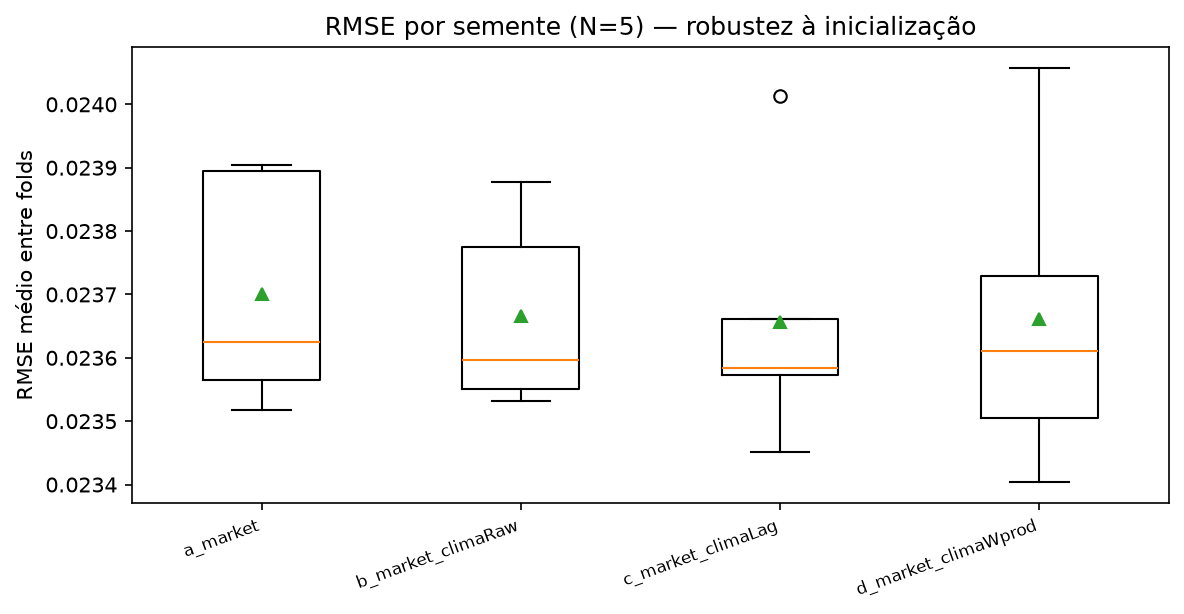
\includegraphics[width=.7\textwidth]{fig_robustez.png}
\caption{RMSE por semente ($N=5$) por configuração. A variabilidade entre sementes é
comparável às diferenças entre configurações.}
\label{fig:robustez}
\end{figure}

\paragraph{Volatilidade.} O GARCH(1,1) não superou consistentemente um benchmark de
variância constante (QLIKE médio $-6{,}508$ vs.\ $-6{,}518$; GARCH vence em 2 de 5
folds). Assim, embora haja \emph{clustering} de volatilidade, ele é difícil de explorar
em previsão de um passo neste período.

\paragraph{Atributos selecionados.} A seleção dentro do fold é estável: além dos
atributos de mercado (\texttt{ret\_cafe}, \texttt{sma\_10}, \texttt{vol\_5},
\texttt{vol\_21}, \texttt{ret\_cambio}) e da sazonalidade (\texttt{sin\_doy}), a única
variável climática presente no top-12 em \emph{todos} os folds é a umidade relativa de
Manhuaçu; logo abaixo aparecem temperatura de Patrocínio e precipitação de Manhuaçu.
Isso indica que, quando o clima contribui, ele o faz por estações específicas ---
reforçando o achado de que a granularidade regional importa.

\paragraph{Discussão.} A Figura~\ref{fig:comparativo} sintetiza MASE e acurácia
direcional. O conjunto de evidências aponta para um mercado próximo à eficiência na
média diária~\cite{fama1970efficient}: nem modelos lineares (ARIMA) nem não lineares
(LSTM) batem o random walk de forma significativa. A contribuição do clima existe, mas é marginal e não robusta.
Do ponto de vista agroinformático, o resultado relevante é que a \emph{forma} de
representar o clima regional altera o desempenho, e que a resolução por cidade preserva
sinal que a agregação destrói.

\begin{figure}[ht]
\centering
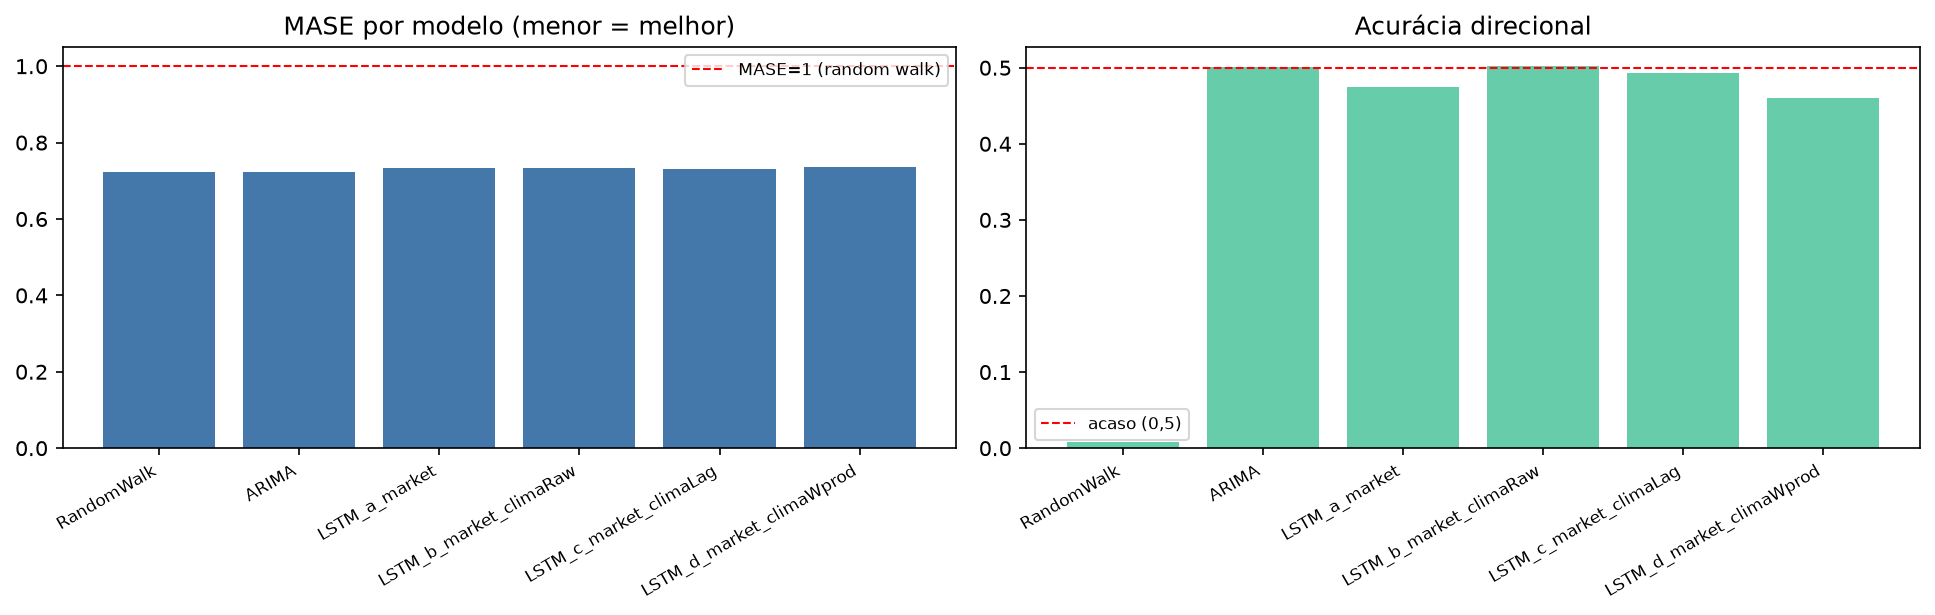
\includegraphics[width=.9\textwidth]{fig_comparativo.png}
\caption{MASE (menor é melhor) e acurácia direcional por modelo. Todas as LSTM ficam
próximas do random walk; apenas a Opção B ultrapassa o acaso na direção.}
\label{fig:comparativo}
\end{figure}

\section{Conclusão}

Apresentamos um estudo rigoroso e reprodutível de previsão do retorno diário do café
arábica combinando mercado e clima regional de Minas Gerais. Sob um protocolo temporal
com controle de vazamento, baselines obrigatórios, teste de significância e
\emph{ensembling} de sementes, nenhum modelo supera o random walk de forma
significativa. Ainda assim, o clima reduz marginalmente o erro e melhora o acerto
direcional, e a representação \emph{por cidade} supera a agregação ponderada por
produção, evidenciando que a granularidade regional carrega sinal útil. Como trabalhos
futuros, destacam-se a busca de hiperparâmetros dentro do fold, horizontes de previsão
mais longos (onde efeitos climáticos defasados podem ser mais visíveis) e a avaliação por
métricas econômicas (simulação de estratégia direcional).

\section*{Agradecimentos}

Ao IFMG -- Campus Bambuí pelo apoio. Aos provedores dos dados públicos INMET e Yahoo
Finance.

\bibliographystyle{sbc}
\bibliography{sbc-template}

\end{document}
